\Chapter{Bewegungsspiele}
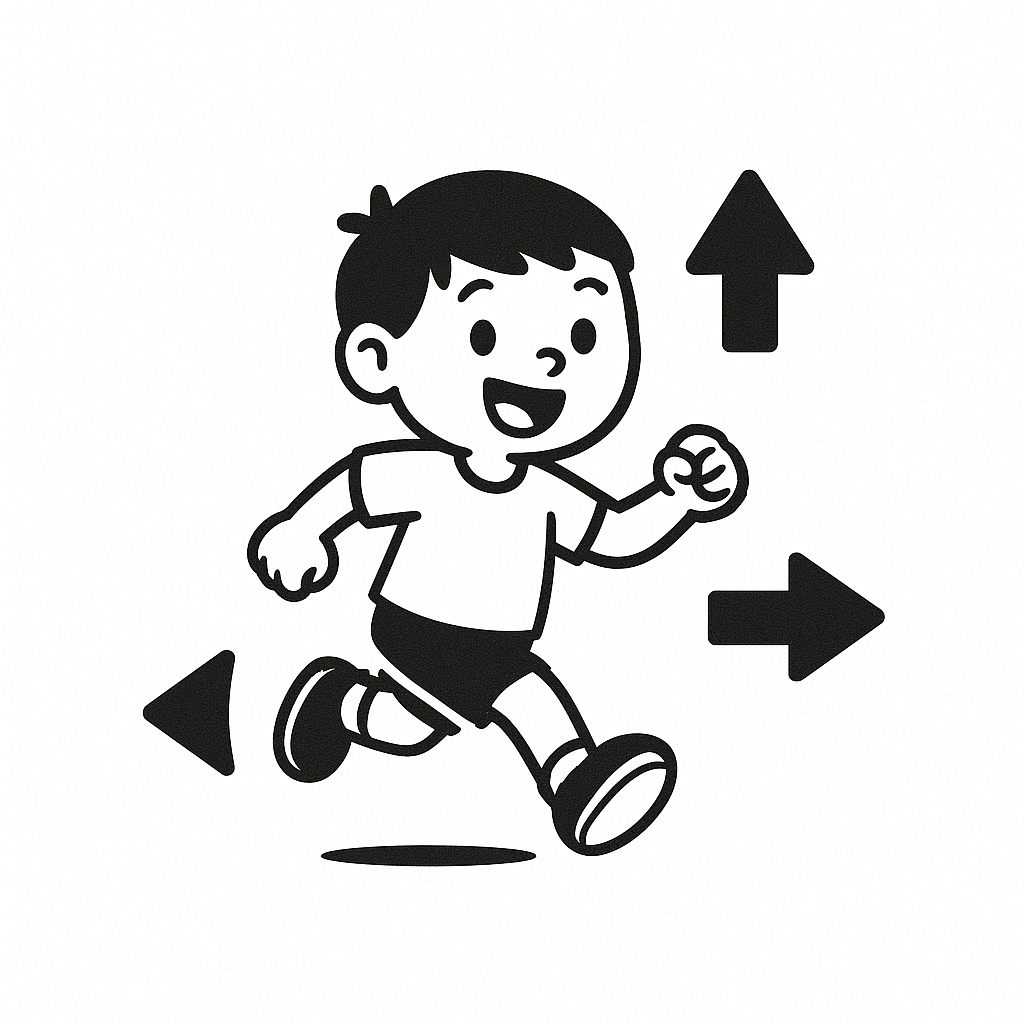
\includegraphics[scale=0.4]{Bilder Kapitel/Bewegungsspiele.png}
%\addthumb{Bewegungsspiele}{\space\Huge\sffamily\bfseries \thechapter}{white}{bbe}
\newpage
%%%%%%%%%%%%%%%%%%%%%%%%%%%%%%%%%%%%%%%%%%%%%%%%%%%%%%%%%%%%%%%%%%%%%%%%%%%%%%%%%%%%%%%%%%%%%%%%%%%%
%Der Fisch muss vom Tisch
%%%%%%%%%%%%%%%%%%%%%%%%%%%%%%%%%%%%%%%%%%%%%%%%%%%%%%%%%%%%%%%%%%%%%%%%%%%%%%%%%%%%%%%%%%%%%%%%%%%%
\Section{Der Fisch muss vom Tisch}
\begin{table}[H]
\begin{tabular}{>{\bfseries}lp{8cm}}
   Gruppengröße:   & 6-15 Spieler*innen\\
    Alter: & 8 \\
    Material: & Streichhölzer, Würfel \\
\end{tabular}
\end{table} 
Die Streichhölzer sind die Fische, von denen jeder Mitspieler 20 Stück vor sich liegen hat. Nach einer „Leerrunde“, bei der die höchste Augenzahl gewinnt und damit bestimmt, wer anfangen darf, geht es richtig los. Dann muss nämlich je der versuchen, seine Fische so schnell wie möglich loszuwerden. Wer als Erster einen blanken (leeren) Tisch anmelden kann, hat gewonnen!

Am Anfang geht es ganz flott: Bei jedem Wurf darf diejenige Anzahl an Streichhölzern weggelegt werden, die der Anzahl der Würfelaugen entspricht. Wirft jemand eine „5“, ister fünf Fische los. Wirft jemand eine „3“, darf er drei Stück zur Seite legen usw. Schwierig wird es, wenn der Fischbestand auf weniger als sechs Stück zusammengeschrumpft ist. Würfelt nämlich jemand eine 5, hat aber nur noch vier Fische vor sich liegen, muss er sich einen dazu holen. Dem Nachbarn ergeht es vielleicht noch schlechter, denn er hatte sich möglicherweise schon auf einen einzigen Fisch heruntergewirtschaftet und würfelt eine 6. Dann kommen gleich 5 Fische inden eigenen Bestand zurück.Das Ziel ist es natürlich alle Fische loszuwerden. \\



%%%%%%%%%%%%%%%%%%%%%%%%%%%%%%%%%%%%%%%%%%%%%%%%%%%%%%%%%%%%%%%%%%%%%%%%%%%%%%%%%%%%%%%%%%%%%%%%%%%%
%Nase auf Blau 
%%%%%%%%%%%%%%%%%%%%%%%%%%%%%%%%%%%%%%%%%%%%%%%%%%%%%%%%%%%%%%%%%%%%%%%%%%%%%%%%%%%%%%%%%%%%%%%%%%%%
\Section{Nase auf Blau}
\begin{table}[H]
\begin{tabular}{>{\bfseries}lp{8cm}}
  Gruppengröße:   & 6-99 Spieler*innen\\
    Alter: & 8 \\
    Material: & Kein Material nötig \\ 
\end{tabular}
\end{table} 
Ein Spieler beginnt und gibt ein Kommando, das aus einem Körperteil, der Präposition „auf“ und einer Farbe besteht, z.B. Naseauf Blau (Knie auf Grau, Schulter auf Pink...). Sofort müssen sich alle Spieler etwas Blaues im Raum suchen und ihre Nase daranhalten(Kleidungsstücke zählen auch!). Wer zuletzt seine  Nasean etwas Blaues gehalten hat, bekommt einen Minuspunktund darf das  nächste Kommando geben. \\




%%%%%%%%%%%%%%%%%%%%%%%%%%%%%%%%%%%%%%%%%%%%%%%%%%%%%%%%%%%%%%%%%%%%%%%%%%%%%%%%%%%%%%%%%%%%%%%%%%%%
%Evolution
%%%%%%%%%%%%%%%%%%%%%%%%%%%%%%%%%%%%%%%%%%%%%%%%%%%%%%%%%%%%%%%%%%%%%%%%%%%%%%%%%%%%%%%%%%%%%%%%%%%%
\Section{Evolution}
\begin{table}[H]
\begin{tabular}{>{\bfseries}lp{8cm}}
   Gruppengröße:   & 10-99 Spieler*innen\\
    Alter: & 8 \\
    Material: & Kein Material nötig \\
\end{tabular}
\end{table} 

    Alle Spieler starten mit der ersten Evolutionsstufe und laufen herum. Treffensich zwei gleiche Evolutionsstufen, führen sie ein Duell in „Schere, Stein, Papier“durch. Der Gewinner steigt eine Stufe auf, der Verlierer bleibt in der Evolutionsstufe. Ziel ist es, die letzte Stufe zu erreichen. Wenn alle richtig gespielt haben, bleibt am Ende je ein Vertreter jeder Stufe von 1-4übrig. Es gibt folgenden Evolutionsstufen:
    \begin{enumerate}
        \item Ei –in der Hocke laufen, sich mit der Hand auf den Kopf schlagen und „Ei  Ei Ei Ei Ei...“ rufen
        \item Huhn –bekannte Hühnerbewegung und gackern
        \item Dino –mit beiden Armen ein großes Dinomaul nachahmen und dabei wie ein Dino schreien. 
        \item Ritter –Mit dem Schwert herumfuchteln und dabei immer wieder rufen „Ich schlage dich, du Schuft“
        \item Weise/r Mann/Frau –an den Rand des Geschehens stellen und sich den Bart streicheln
        
    \end{enumerate}
    Tipp: Es empfiehlt sich, die Evolutionsstufenim Vorfeld gemeinsam zu üben.




%%%%%%%%%%%%%%%%%%%%%%%%%%%%%%%%%%%%%%%%%%%%%%%%%%%%%%%%%%%%%%%%%%%%%%%%%%%%%%%%%%%%%%%%%%%%%%%%%%%%
%Kettenkrieger 
%%%%%%%%%%%%%%%%%%%%%%%%%%%%%%%%%%%%%%%%%%%%%%%%%%%%%%%%%%%%%%%%%%%%%%%%%%%%%%%%%%%%%%%%%%%%%%%%%%%%
\Section{Kettenkrieger}

\begin{table}[H]
\begin{tabular}{>{\bfseries}lp{8cm}}
  Gruppengröße:   & 12-99 Spieler*innen\\
    Alter: & 8 \\
    Material: & Kein Material nötig \\ 
\end{tabular}
\end{table} 


Ein Spieler ist der erste Ticker und muss andere Spieler versuchen zu fangen.  Alle anderen laufen dabei weg. Wird ein Spieler gefangen, so müssen sich die Beiden „aneinander ketten“ (d.h. sie halten sich an den Händen fest). Die „Kette“ (die beiden Spieler) muss jetzt versuchen andere Spieler zu fangen, dabei dürfen sie sich nicht loslassen. Die „Kette“ wird durch jeden gefangenen Spielerlänger, bis nur noch eine Person überbleibt und dann eine neue Spielrunde beginnt.  \\ \newline
    Variation: \\ Eine Kette besteht maximal aus drei Personen. Kommt eine vierte Person hinzu, teilt sich die Gruppe in zwei 2er Gruppen. Jetzt ticken zwei Ketten.\\


%%%%%%%%%%%%%%%%%%%%%%%%%%%%%%%%%%%%%%%%%%%%%%%%%%%%%%%%%%%%%%%%%%%%%%%%%%%%%%%%%%%%%%%%%%%%%%%%%%%%
%Zombieball
%%%%%%%%%%%%%%%%%%%%%%%%%%%%%%%%%%%%%%%%%%%%%%%%%%%%%%%%%%%%%%%%%%%%%%%%%%%%%%%%%%%%%%%%%%%%%%%%%%%%
\Section{Zombieball}


\begin{table}[H]
\begin{tabular}{>{\bfseries}lp{8cm}}
   Gruppengröße:   & 6-99 Spieler*innen\\
    Alter: & 8 \\
    Material: & Kein Material nötig \\ 
\end{tabular}
\end{table} 
 In dem Spiel spielt jeder gegen jeden. Es wird ein Ball ins Spiel gegeben und die Spieler müssen versuchen den Ball für sich zu gewinnen, damit sie möglichst viele andere Mitspieler abtreffen können. Hierbei ist zu beachten, dass man entweder dem Ball ausweicht oder den Ball fängt. Wenn man den Ball fängt,bleibt man im Spielfeld und wenn man abgeworfen wird, setzt man sich am Rand z.B. auf eine Bank hin.Jeder abgeworfene Spieler muss sich merken, wer ihn abgeworfen hat, da er sobald dieser von einem anderen abgeworfen wird, wieder auf das Spielfeld darf. Bei diesem Spiel ist es so, dass man nicht gleich aus dem Spiel ausgeschieden ist, wenn man getroffen wird. Man kann immer wieder sein Geschick unter Beweis stellen. \\ \newline
    Variante: \\ Durch einen zweiten Ball kann die Schwierigkeit erhöht werden.\\


\newpage
%%%%%%%%%%%%%%%%%%%%%%%%%%%%%%%%%%%%%%%%%%%%%%%%%%%%%%%%%%%%%%%%%%%%%%%%%%%%%%%%%%%%%%%%%%%%%%%%%%%%
%Riese, Elfen, Zauberer
%%%%%%%%%%%%%%%%%%%%%%%%%%%%%%%%%%%%%%%%%%%%%%%%%%%%%%%%%%%%%%%%%%%%%%%%%%%%%%%%%%%%%%%%%%%%%%%%%%%%
\Section{Riese, Elfen, Zauberer}

\begin{table}[H]
\begin{tabular}{>{\bfseries}lp{8cm}}
   Gruppengröße:   & 10-99 Spieler*innen\\
    Alter: & 8 \\
    Material: & Kein Material nötig \\
\end{tabular}
\end{table} 
 Bei diesem Spiel gibt es drei Figuren, von denen eine immer stärker ist als die andere. Die Spieler teilen sich in zwei Gruppen auf. Sie überlegen sich innerhalb einer Gruppe, welche Figur sie darstellen wollen (ohne dass die andere Gruppe mithört). Dann stellen sich die beiden Gruppen in einer langen Reihe zueinander auf, der Abstand zwischen den beiden Gruppen soll ca. 1 m betragen. Auf ein Signal des Spielleiters stellen beide Gruppen ihre Figur dar. Die Gruppe, die die stärkere Figur hat, muss möglichst viele Leute aus der anderen Gruppe fangen.  Die „schwächere“ Gruppe muss zum Ende des Spielfeldes laufen, um „sicher“ zu sein. Das Spiel kann solange gespielt werden, bis alle in einer Gruppe sind.\newline

Rollen zum Spiel: Riesen:Sie stellen sich auf Zehenspitzen, strecken die Arme in die Luft, schauen grimmig und brüllen laut: „Riesen!“ Elfen:Elfen machen sich klein, ziehen die Schulter ein und flüstern ganz leise:  „Elfen“ Zauberer:Sie haben einen buckligen Rücken, magischen Blick und zischen mit verzaubernden Gesten „Zauberer!“\newline

Wichtig: Die Riesen sind stärker als die Elfen; die Elfen sind stärker als die Zauberer; die Zauberer sind stärker als die Riesen \\



%%%%%%%%%%%%%%%%%%%%%%%%%%%%%%%%%%%%%%%%%%%%%%%%%%%%%%%%%%%%%%%%%%%%%%%%%%%%%%%%%%%%%%%%%%%%%%%%%%%%
%Kegelfußball 
%%%%%%%%%%%%%%%%%%%%%%%%%%%%%%%%%%%%%%%%%%%%%%%%%%%%%%%%%%%%%%%%%%%%%%%%%%%%%%%%%%%%%%%%%%%%%%%%%%%%
\Section{Kegelfußball}

\begin{table}[H]
\begin{tabular}{>{\bfseries}lp{8cm}}
   Gruppengröße:   & Ab 6 Spieler*Innen\\
    Alter: & 5 \\
    Material: & Pro Personen einen Kegel, einen Fußball  \\
\end{tabular}
\end{table} 

 Jedes Kind erhält einen Kegel. Alle Mitspieler verteilen sich in der Halle und stellen ihre Kegel dort ab. Nun legt der Spielleiter einen Fußball in die Mitte der Halle und eröffnet das Spiel. Bei vielen Spielern kann man auch zwei oder drei Bälle einsetzen. Nun versucht jeder Spieler die Kegel der anderen Mitspieler um zuschießen. Fällt der eigene Kegel um, ist man ausgeschieden. Ebenfalls scheidet man aus, wenn man seinen eigenen Kegel, z.B. aus Versehen beim Verteidigen, umstößt. Am Ende bleiben nur noch 2 Spieler übrig. Gewonnen hat derjenige, dessen Kegel am Ende noch steht.
 \\ \newline
 Variation: \\ Das Spiel kann man auch gegeneinander spielen. Es werden zwei Teams gebildet und man stellt die Kegel gegenüber voneinander auf (z.B. in einem Abstand von 6m). Beide Teams versuchen die Kegel der gegnerischen Mannschaft um zuschießen. Gewonnen hat die Mannschaft, die zuerst alle Kegel der gegnerischen Mannschaft um geschossen hat.\\


\newpage
%%%%%%%%%%%%%%%%%%%%%%%%%%%%%%%%%%%%%%%%%%%%%%%%%%%%%%%%%%%%%%%%%%%%%%%%%%%%%%%%%%%%%%%%%%%%%%%%%%%%
%Buchstabenbelegen
%%%%%%%%%%%%%%%%%%%%%%%%%%%%%%%%%%%%%%%%%%%%%%%%%%%%%%%%%%%%%%%%%%%%%%%%%%%%%%%%%%%%%%%%%%%%%%%%%%%%
\Section{Buchstabenbelegen}


\begin{table}[H]
\begin{tabular}{>{\bfseries}lp{8cm}}
   Gruppengröße:   & 15-30 Spieler*innen\\
    Alter: & 8 \\
    Material: & Buchstabenkarten von A bis Z pro Gruppe \\ 
\end{tabular}
\end{table} 

 Die Gesamtgruppe wird in Kleingruppen (4-6 Personen) getrennt. Jede Klein Gruppe erhält das Alphabet als Buchstabenkarten (jeder Buchstabe auf einem Blatt Papier). Auf Kommando beginnt das Spiel. Ziel ist es, auf jede Karte einen Gegenstand zu legen, der mit diesem Anfangsbuchstaben beginnt. Es ist auch Kreativität gefragt, z.B. zählt bei C auch „Christianes Uhr“ oder bei U „unsichtbarer Kugelschreiber“. Die Gruppe, die zuerst fertig ist, hat gewonnen. \\



%%%%%%%%%%%%%%%%%%%%%%%%%%%%%%%%%%%%%%%%%%%%%%%%%%%%%%%%%%%%%%%%%%%%%%%%%%%%%%%%%%%%%%%%%%%%%%%%%%%%
%Kartenlauf
%%%%%%%%%%%%%%%%%%%%%%%%%%%%%%%%%%%%%%%%%%%%%%%%%%%%%%%%%%%%%%%%%%%%%%%%%%%%%%%%%%%%%%%%%%%%%%%%%%%%
\Section{Kartenlauf}

\begin{table}[H]
\begin{tabular}{>{\bfseries}lp{8cm}}
   Gruppengröße:   & 12-99 Spieler*innen\\
    Alter: & 6 \\
    Material: & Kartenspiel \\
\end{tabular}
\end{table} 

Zur Vorbereitung werden alle Karten des Spiels verdeckt in der Mitte der Halle gelegt. Die Spieler stehen in 4 Gruppen an jeder Ecke der Halle und erhalten durch Losentscheid eine der 4 Asse (Karo, Herz, Kreuz oder Pik).
Auf Kommando beginnt das Spiel. Der jeweils Erste jeder Gruppe läuft in die Mitte und dreht eine beliebige Karte um. Ist sie von seiner Farbe, darf er sie mitnehmen. Ist die Karte nicht von seiner Farbe, dreht er sie wieder um. Er sprintet zurück zu seiner Gruppe, schlägt per Handschlag ab und der nächste Läufer darf starten. Das wiederholt sich in jeder Gruppe solange, bis alle Karten einer Farbe gesammelt wurden (2, 3, 4, 5, 6, 7, 8, 9, 10, Bube, Dame, König und Ass). Sieger ist die Mannschaft, welche zuerst alle Karten ihrer Farbe komplett hat.
 \\ \newline
 Variante 1: \\ Es wird mit weniger Karten gespielt.\\
 Variante 2: \\ Es muss der Reihe nach gesammelt werden (Straße). ACHTUNG: dauert sehr lange und ist eher für Ältere gedacht.\\
 



%%%%%%%%%%%%%%%%%%%%%%%%%%%%%%%%%%%%%%%%%%%%%%%%%%%%%%%%%%%%%%%%%%%%%%%%%%%%%%%%%%%%%%%%%%%%%%%%%%%%
%Cola, Fanta, Sprite
%%%%%%%%%%%%%%%%%%%%%%%%%%%%%%%%%%%%%%%%%%%%%%%%%%%%%%%%%%%%%%%%%%%%%%%%%%%%%%%%%%%%%%%%%%%%%%%%%%%%
\Section{Cola, Fanta, Sprite}

\begin{table}[H]
\begin{tabular}{>{\bfseries}lp{8cm}}
  Gruppengröße:   & 6-30 Spieler*innen\\
    Alter: & 8 \\
    Material: & Kein Material nötig \\ 
\end{tabular}
\end{table} 
 Ein Streifen Kreppband wird auf den Boden geklebt. Alle Spieler stellen sich schulterbreit auf die Linie. Dann sagt der Spielleiter „Cola“ und alle springen auf die rechte Seite der Linie. Danach sagt der Spielleiter „Sprite“ und alle stellen sich wieder in die Mitte der Linie. Dann sagt er „Fanta“ und alle springen auf die Linke Seite der Linie. Die Begriffe „Cola, Fanta, Sprite“ können natürlich auch in einer x-beliebigen Reihenfolge gerufen werden. Der, der falsch steht, scheidet aus. Als erschwerter Faktor kommt „Mezzo Mix“ hinzu, dabei muss man mit den Beinen gekreuzt auf der Linie stehen. \\




%%%%%%%%%%%%%%%%%%%%%%%%%%%%%%%%%%%%%%%%%%%%%%%%%%%%%%%%%%%%%%%%%%%%%%%%%%%%%%%%%%%%%%%%%%%%%%%%%%%%
%Krabbencatchen
%%%%%%%%%%%%%%%%%%%%%%%%%%%%%%%%%%%%%%%%%%%%%%%%%%%%%%%%%%%%%%%%%%%%%%%%%%%%%%%%%%%%%%%%%%%%%%%%%%%%
\Section{Krabbencatchen}

\begin{table}[H]
\begin{tabular}{>{\bfseries}lp{8cm}}
   Gruppengröße:   & 6-99 Spieler*innen\\
    Alter: & 8 \\
    Material: & Kein Material nötig \\
\end{tabular}
\end{table} 


 Bei diesem Spiel spielen alle Mitspieler gegeneinander. Es gilt, wie Krabben auf allen Vieren zu laufen. Außer den Händen und den Füßen darf kein anderer Körperteil den Boden berühren. Aufstehen ist ebenso wenig erlaubt.Die Aufgabe ist es nun, durchstoßen, schubsen und drücken die anderen Krabben dazu zu bringen, dass sie auf ihrem Gesäß landen oder umfallen. Wer nicht mehr in der Krabbenposition läuft und umgeschubst wurde, scheidet aus und muss die Spielfläche verlassen Wem gelingt es am längsten als Krabbe zu überleben?Die Spielleitung sollte bei diesem Spiel ein besonders waches Auge haben, damit niemand zu stark andere schubst und ärgert. Zu starke Kabbeleien sollten unterbunden werden. \\


%%%%%%%%%%%%%%%%%%%%%%%%%%%%%%%%%%%%%%%%%%%%%%%%%%%%%%%%%%%%%%%%%%%%%%%%%%%%%%%%%%%%%%%%%%%%%%%%%%%%
%Wäscheklammern klauen
%%%%%%%%%%%%%%%%%%%%%%%%%%%%%%%%%%%%%%%%%%%%%%%%%%%%%%%%%%%%%%%%%%%%%%%%%%%%%%%%%%%%%%%%%%%%%%%%%%%%
\Section{Wäscheklammern klauen}

\begin{table}[H]
\begin{tabular}{>{\bfseries}lp{8cm}}
  Gruppengröße:   & 6-30 Spieler*innen\\
    Alter: & 5 \\
    Material: & Für jeden Mitspieler drei oder mehr Wäscheklammern \\
\end{tabular}
\end{table} 
 Jeder Mitspieler bekommt drei Wäscheklammern, die er an seiner Kleidung befestigt. Nach einem Startsignal versuchen sich die Mitspieler gegenseitig die Wäscheklammern zu klauen, um sie bei sich zu befestigen. Wer keine Wäscheklammern mehr hat, scheidet aus. Gewonnen hat, wer nach einer bestimmten Zeitspanne die meisten Wäscheklammern gesammelt hat. \\



%%%%%%%%%%%%%%%%%%%%%%%%%%%%%%%%%%%%%%%%%%%%%%%%%%%%%%%%%%%%%%%%%%%%%%%%%%%%%%%%%%%%%%%%%%%%%%%%%%%%
%Flöhe fangen
%%%%%%%%%%%%%%%%%%%%%%%%%%%%%%%%%%%%%%%%%%%%%%%%%%%%%%%%%%%%%%%%%%%%%%%%%%%%%%%%%%%%%%%%%%%%%%%%%%%%
\Section{Flöhe fangen}

\begin{table}[H]
\begin{tabular}{>{\bfseries}lp{8cm}}
   Gruppengröße:   & 6-15 Spieler*innen\\
    Alter: & 8 \\
    Material: & Augenbinde \\
\end{tabular}
\end{table} 

Alle Spieler sind Flöhe. Einer davon ist der Fänger, ihm werden die Augen verbunden. Wichtig ist, dass sowohl aktive als auch ausgeschiedene Spieler möglichst leise sind, ansonsten ist das Spiel schwer durchführbar.Die Flöhe verteilen sich im Raum und hocken sich nieder. Der Fänger hüpft nun -blind-herum und versucht, die anderen Flöhe durch berühren zu fangen. Wer gefangen ist, stellt sich an eine Seite des Raumes.Durch Weghüpfen können sich die Flöhe auch aus der Gefahrenzone befreien. Allerdings Achtung: jeder Floh darf nur eine vorher definierte Anzahl an Sprüngen vollziehen (etwa 3-5).Dies gilt natürlich nicht für den fangenden Floh, der eine beliebige Anzahl an Sprüngen durchführen kann. \\



%%%%%%%%%%%%%%%%%%%%%%%%%%%%%%%%%%%%%%%%%%%%%%%%%%%%%%%%%%%%%%%%%%%%%%%%%%%%%%%%%%%%%%%%%%%%%%%%%%%%
%Bambule 
%%%%%%%%%%%%%%%%%%%%%%%%%%%%%%%%%%%%%%%%%%%%%%%%%%%%%%%%%%%%%%%%%%%%%%%%%%%%%%%%%%%%%%%%%%%%%%%%%%%%
\Section{Bambule}
\begin{table}[H]
\begin{tabular}{>{\bfseries}lp{8cm}}
   Gruppengröße:   & 12-99 Spieler*innen\\
    Alter: & 8 \\
    Material: & Absperrband, Socke mit Tennisball \\
\end{tabular}
\end{table} 
 Es wird ein Spielfeld abgesteckt ca. 10x10 Meter. Jeder Spieler bekommt eine Nummer zugeordnet, am besten auf einen Kreppklebestreifen schreiben. Anschließend teilt sich die Gruppe auf die vier Seiten auf. Der Spielleiter liest immer zwei Nummernaus einem gegenüberliegenden Team vor, die dann versuchen müssen, die Socke auf ihre Seite zubringen.  Der Kampf um die Socke gilt als gewonnen, sobald die Socke über der abgesperrten Linie ist. 
WICHTIG: Darauf achten, dass die Kinder alle angemessene Kleidung anhaben und die Kämpfe nicht zu stark werden.\\



%%%%%%%%%%%%%%%%%%%%%%%%%%%%%%%%%%%%%%%%%%%%%%%%%%%%%%%%%%%%%%%%%%%%%%%%%%%%%%%%%%%%%%%%%%%%%%%%%%%%
%Glucke, Küken, Fuchs
%%%%%%%%%%%%%%%%%%%%%%%%%%%%%%%%%%%%%%%%%%%%%%%%%%%%%%%%%%%%%%%%%%%%%%%%%%%%%%%%%%%%%%%%%%%%%%%%%%%%
\Section{Glucke, Küken, Fuchs}
\begin{table}[H]
\begin{tabular}{>{\bfseries}lp{8cm}}
   Gruppengröße:   & 6-30 Spieler*innen\\
    Alter: & 8 \\
    Material: & Kein Material nötig \\ 
\end{tabular}
\end{table} 
Die Teilnehmer stellen sich in zwei Kreise voreinander auf. Eine Person sollte übrig sein und stellt den Fuchs da. Die Person im hinteren Kreis sind die Küken und im vorderen die Glucken. Die Glucken versuchen mit lautem Gegacker die Küken zu retten und den Fuchs zu verscheuchen. Der Fuchs versucht an die Küken dran zu kommen. Beidem Spiel geht es darum zu lernen wie man sich für einander stark macht. 
 \\



%%%%%%%%%%%%%%%%%%%%%%%%%%%%%%%%%%%%%%%%%%%%%%%%%%%%%%%%%%%%%%%%%%%%%%%%%%%%%%%%%%%%%%%%%%%%%%%%%%%%
%Jeder fängt jeden
%%%%%%%%%%%%%%%%%%%%%%%%%%%%%%%%%%%%%%%%%%%%%%%%%%%%%%%%%%%%%%%%%%%%%%%%%%%%%%%%%%%%%%%%%%%%%%%%%%%%
\Section{Jeder fängt jeden}
\begin{table}[H]
\begin{tabular}{>{\bfseries}lp{8cm}}
   Gruppengröße:   & 6-40 Spieler*innen\\
    Alter: & 8 \\
    Material: & Kein Material nötig  \\
\end{tabular}
\end{table} 

 Alle spielen gegeneinander. Jeder darf jeden ticken. Die getickten müssen stehen bleiben und sich merken von wem sie getickt worden sind.  Wird diese Person dann getickt, ist man selber wieder frei. \\


%%%%%%%%%%%%%%%%%%%%%%%%%%%%%%%%%%%%%%%%%%%%%%%%%%%%%%%%%%%%%%%%%%%%%%%%%%%%%%%%%%%%%%%%%%%%%%%%%%%%
%Fangen im Gehen
%%%%%%%%%%%%%%%%%%%%%%%%%%%%%%%%%%%%%%%%%%%%%%%%%%%%%%%%%%%%%%%%%%%%%%%%%%%%%%%%%%%%%%%%%%%%%%%%%%%%
\Section{Fangen im Gehen}
\begin{table}[H]
\begin{tabular}{>{\bfseries}lp{8cm}}
   Gruppengröße:   & 6-99 Spieler*innen\\
    Alter: & 10 \\
    Material: & Kein Material nötig \\
\end{tabular}
\end{table} 

 Jeder Spieler bekommt einen Partner zugelost.  Der eine wird zum Fänger der andere zum gejagt, doch für beide gilt, man darf nicht anfangen zu rennen, sondern nur laufen! Man kann auch sagen, dass man nur Rückwärts gehen darf oder humpelnd Erweiterung: Alle Spieler rennen wild Durcheinander und versuchen dabei die anderen nicht zu berühren. Wenn dies aber doch passiert muss drei Mal ganz laut geflucht werden. Das Spielfeld kann man immer kleiner machen. \\



%%%%%%%%%%%%%%%%%%%%%%%%%%%%%%%%%%%%%%%%%%%%%%%%%%%%%%%%%%%%%%%%%%%%%%%%%%%%%%%%%%%%%%%%%%%%%%%%%%%%
%Drachenschwanzjagd
%%%%%%%%%%%%%%%%%%%%%%%%%%%%%%%%%%%%%%%%%%%%%%%%%%%%%%%%%%%%%%%%%%%%%%%%%%%%%%%%%%%%%%%%%%%%%%%%%%%%
\Section{Drachenschwanzjagd}
\begin{table}[H]
\begin{tabular}{>{\bfseries}lp{8cm}}
   Gruppengröße:   & 6-99 Spieler*innen\\
    Alter: & 6 \\
    Material: & Reepschnur bzw. Tuch als Schwanz \\
\end{tabular}
\end{table} 

Alle Kinder stehen in einer Schlange hintereinander und fassen mit den Händen um die Hüfte des Vordermanns. Der Letzte (=Schwanz) hat eine Reepschnur/ein Tuch etc. in seiner Hose als Schwanz stecken. Der Erste (=Drachen-Kopf) muss den Schwanz abreißen, ohne dass sein „Körper“ (= restliche Kinder) auseinanderfällt. Hat er es geschafft, kommt der Erste an die letzte Stelle, und so weiter.
 \\ \newline
 Variante: \\ 2 Drachen\\



%%%%%%%%%%%%%%%%%%%%%%%%%%%%%%%%%%%%%%%%%%%%%%%%%%%%%%%%%%%%%%%%%%%%%%%%%%%%%%%%%%%%%%%%%%%%%%%%%%%%
%Bierdeckel werfen
%%%%%%%%%%%%%%%%%%%%%%%%%%%%%%%%%%%%%%%%%%%%%%%%%%%%%%%%%%%%%%%%%%%%%%%%%%%%%%%%%%%%%%%%%%%%%%%%%%%%
\Section{Bierdeckel werfen}
\begin{table}[H]
\begin{tabular}{>{\bfseries}lp{8cm}}
   Gruppengröße:   & 6-99 Spieler*innen\\
    Alter: & 6 \\
    Material: & Bierdeckel \\
\end{tabular}
\end{table} 


    Man steckt ein Feld ab und bildet zwei Mannschaften.  Jetzt sucht man sich eine Spiel Variante raus.
    \begin{enumerate}
        \item Variante: Bierdeckel ins gegnerische Feld werfen
        \item Variante: Bierdeckel umdrehen, jede Mannschaft muss alle seinen Bierdeckel auf eine Seite gedreht bekommen
        \item Variante: Die Bierdeckel müssen aufgesammelt werden, wer am Ende die meisten hat, hat gewonnen.
    \end{enumerate}
    Die Ideen Mannschaftsspiele aus Bierdeckel zu machen, kann man individuell überlegen. 
    \\


%%%%%%%%%%%%%%%%%%%%%%%%%%%%%%%%%%%%%%%%%%%%%%%%%%%%%%%%%%%%%%%%%%%%%%%%%%%%%%%%%%%%%%%%%%%%%%%%%%%%
%Lifter
%%%%%%%%%%%%%%%%%%%%%%%%%%%%%%%%%%%%%%%%%%%%%%%%%%%%%%%%%%%%%%%%%%%%%%%%%%%%%%%%%%%%%%%%%%%%%%%%%%%%
\Section{Lifter}
\begin{table}[H]
\begin{tabular}{>{\bfseries}lp{8cm}}
   Gruppengröße:   & 6-99 Spieler*innen\\
    Alter: & 6 \\
    Material: & Kein Material nötig \\
\end{tabular}
\end{table} 
Alle Kinder, bis auf eins, stehen auf einer Seite, die andere Person steht gegenüber mit ca. 30 Meter Abstand. Jetzt ruft die einzelne Person „Wer hat Angst vorm Lifter“, die Gruppe antwortet mit „Niemand“, dann der Lifter „und wenn er kommt“ „dann rennen wir“ Jetzt rennen die Personen los, der Lifter hat die Aufgabe Personen hochzuheben, wenn er es bei einer Person geschafft hat, wird diese auch zum Lifter und helfen dem Lifter in der nächsten Runde beim liften.  \\



%%%%%%%%%%%%%%%%%%%%%%%%%%%%%%%%%%%%%%%%%%%%%%%%%%%%%%%%%%%%%%%%%%%%%%%%%%%%%%%%%%%%%%%%%%%%%%%%%%%%
%Tortenvölkerball
%%%%%%%%%%%%%%%%%%%%%%%%%%%%%%%%%%%%%%%%%%%%%%%%%%%%%%%%%%%%%%%%%%%%%%%%%%%%%%%%%%%%%%%%%%%%%%%%%%%%
\Section{Tortenvölkerball}
\begin{table}[H]
\begin{tabular}{>{\bfseries}lp{8cm}}
   Gruppengröße:   & 6-99 Spieler*innen\\
    Alter: & 6 \\
    Material: & Kein Material nötig \\ 
\end{tabular}
\end{table} 
 Spielerklärung
Etwas zum Abstecken des Spielfeldes, Bälle Es wird ein rundes Spielfeld abgesteckt, mit einem kleinen extra Kreis drum herum. Dann wird der Kreis in 6 Stücke aufgeteilt.  Die Spielleiter*in muss jetzt 6 Mannschaften bilden. Jede Mannschaft bestimmt einen Hintermann/frau (der letzte Spieler, der 3 Leben hat). Die restlichen Spieler sind in ihrem Tortenstück und werfen sich gegenseitig mit Bällen ab. Wenn einer getroffen worden ist,dann muss er zum Hintermann ins Feld. Er kann sich wieder frei werfen, indem er eine Person auf dem Feld trifft.Man darf nur seine Nachbarfelder abwerfen und nicht über andere Felder drüber werfen. \\



%%%%%%%%%%%%%%%%%%%%%%%%%%%%%%%%%%%%%%%%%%%%%%%%%%%%%%%%%%%%%%%%%%%%%%%%%%%%%%%%%%%%%%%%%%%%%%%%%%%%
%Hase und Igel
%%%%%%%%%%%%%%%%%%%%%%%%%%%%%%%%%%%%%%%%%%%%%%%%%%%%%%%%%%%%%%%%%%%%%%%%%%%%%%%%%%%%%%%%%%%%%%%%%%%%
\Section{Hase und Igel}
\begin{table}[H]
\begin{tabular}{>{\bfseries}lp{8cm}}
   Gruppengröße:   & 6-99 Spieler*innen\\
    Alter: & 6 \\
    Material: & Kein Material nötig \\
\end{tabular}
\end{table} 

Je zwei Kinder haken sich mit Armen bei einander ein. Diese Zweiergrüppchen verteilen sich auf der Fläche.Zwei Kinder sind Fänger und Gefangener. Gejagter kann sich in Sicherheit bringen, indem er sich bei einem Zweiergrüppchen dazu einhackt. Hat er sich eingehakt, muss sich der äußere dritte von dem Grüppchen lösen und wird nun zum Fänger. Der Fänger wird somit plötzlich zum Gejagten.Kann der Fänger den Gejagten fangen, wechseln ebenfalls die Rollen –der Fänger wird zum Gejagten und umgekehrt.Dieses Spiel ist auch sehr nett als Storch und Bär (statt Hase und Igel). Alles gleich, jedoch ist der Fänger der Bär und muss während dem Fangen laut brüllen und mit den Händen„Bär Kratz-Fang-Bewegungen“ machen.Der Gefangene ist der Storch. Dieser muss mit ausgestreckten Armen vor sich in die Händeklatschen und während dem Rennen laut „klapp –klapp“ rufen. \\



%%%%%%%%%%%%%%%%%%%%%%%%%%%%%%%%%%%%%%%%%%%%%%%%%%%%%%%%%%%%%%%%%%%%%%%%%%%%%%%%%%%%%%%%%%%%%%%%%%%%
%Wo ist mein Huhn
%%%%%%%%%%%%%%%%%%%%%%%%%%%%%%%%%%%%%%%%%%%%%%%%%%%%%%%%%%%%%%%%%%%%%%%%%%%%%%%%%%%%%%%%%%%%%%%%%%%%
\Section{Wo ist mein Huhn}
\begin{table}[H]
\begin{tabular}{>{\bfseries}lp{8cm}}
   Gruppengröße:   & 6-30 Spieler*innen\\
    Alter: & 10 \\
    Material: & Gummihuhn oder ähnliches \\ 
\end{tabular}
\end{table} 

Eine Person wird ausgesucht und entfernt sich ca. 15 Meter von der Gruppe. Das Huhn wird vor diese Person auf den Boden gelegt. Die Gruppe stellt sich in einer Reihe nebeneinander auf. Die auserwählte Person dreht sich um und ruft: „WOOOO...IST...MEIN...HUHN!!“ Dann dreht sich diese wieder zur Gruppe. In dem Zeitraum, wo die Person sich umdreht, darf die Gruppe sich bewegen und versuchen das Huhn zu bekommen. Wenn sich jemand weiterbewegt, nachdem die Person sich wieder umgedreht hat, wird dieser wieder an den Anfang zurückgeschickt. Wenn es jemand geschafft hat, das Huhn zu bekommen ohne dabei gesehen zu werden, muss dieses -ohne es zu werfen -zurück an die \newline
Startlinie gebracht werden. Die Person darf Einzelne aus der Gruppe auswählen, welche auf Befehl die Hände heben müssen und so zeigen, dass sie das Huhn nicht haben. Ziel des Spiels ist es so  unentdeckt das Huhn über die Ziellinie zu bekommen. \\



%%%%%%%%%%%%%%%%%%%%%%%%%%%%%%%%%%%%%%%%%%%%%%%%%%%%%%%%%%%%%%%%%%%%%%%%%%%%%%%%%%%%%%%%%%%%%%%%%%%%
%Das Tütenspiel
%%%%%%%%%%%%%%%%%%%%%%%%%%%%%%%%%%%%%%%%%%%%%%%%%%%%%%%%%%%%%%%%%%%%%%%%%%%%%%%%%%%%%%%%%%%%%%%%%%%%
\Section{Das Tütenspiel}
\begin{table}[H]
\begin{tabular}{>{\bfseries}lp{8cm}}
   Gruppengröße:   & 10-99 Spieler*innen\\
    Alter: & 6 \\
    Material: & Pro Betreuer eine Tüte, gefüllt mit 10 Gegenständen \\ 
\end{tabular}
\end{table} 
Jeder Betreuer bekommt eine Tüte gefüllt mit 10 Gegenständen drin. Die Kinder versuchen nun die Betreuer zu ticken und einen Blick für 10 Sekunden in die Tüte zubekommen und die Gegenstände auf eine Liste zuschrieben. Doch das gemeine ist, das Betreuer untereinander die ganzen Tüten oder auch nur einzelne Gegenstände tauschen dürfen. Auch dürfen die Betreuer vor den Kindern wegrennen. Nach Ablauf der Zeit gewinnt die Gruppe mit den meisten Gegenständen.  \\



%%%%%%%%%%%%%%%%%%%%%%%%%%%%%%%%%%%%%%%%%%%%%%%%%%%%%%%%%%%%%%%%%%%%%%%%%%%%%%%%%%%%%%%%%%%%%%%%%%%%
%Das Chaosspiel
%%%%%%%%%%%%%%%%%%%%%%%%%%%%%%%%%%%%%%%%%%%%%%%%%%%%%%%%%%%%%%%%%%%%%%%%%%%%%%%%%%%%%%%%%%%%%%%%%%%%
\Section{Das Chaosspiel}
\begin{table}[H]
\begin{tabular}{>{\bfseries}lp{8cm}}
   Gruppengröße:   & 10-99 Spieler*innen\\
    Alter: & 6 \\
    Material: & Ein Spielplan, Spielfiguren, Karten mit Nummer und Codewort \\
\end{tabular}
\end{table} 

Auf dem gesamten Gelände sind Karten verteilt mit einer Nummer (1-100) und auf der anderen Seite einem Codewort. Die Kinder müssen Würfeln und haben dann die Aufgabe die Nummer, auf der sie gelandet sind zu suchen, dann bringen sie das Codewort zur Spielleitung und müssen eine kleine Aufgabe erledigen. (Ein Lied singen, Liegestützen, Hampelmänner, irgendetwas bringen etc.) Nach der Erfüllung der Aufgabe, darf die Gruppe erneut würfeln. \\



%%%%%%%%%%%%%%%%%%%%%%%%%%%%%%%%%%%%%%%%%%%%%%%%%%%%%%%%%%%%%%%%%%%%%%%%%%%%%%%%%%%%%%%%%%%%%%%%%%%%
%Muh-Mäh-Miau-Spiel
%%%%%%%%%%%%%%%%%%%%%%%%%%%%%%%%%%%%%%%%%%%%%%%%%%%%%%%%%%%%%%%%%%%%%%%%%%%%%%%%%%%%%%%%%%%%%%%%%%%%
\Section{Muh-Mäh-Miau-Spiel}
\begin{table}[H]
\begin{tabular}{>{\bfseries}lp{8cm}}
   Gruppengröße:   & 12-99 Spieler*innen\\
    Alter: & 6 \\
    Material: & röte, Zettel, Stift \\
\end{tabular}
\end{table} 

 Die Betreuer haben eine Liste von Tiergeräuschen, die sie machen müssen, Sie verteilen sich auf dem Gelände und laufen durch die Gegend.  Nach jeweils 5 Minuten ertönt ein Geräusch, das zum Tierwechsel ruft. Die Kinder müssen alle Tiere finden. Um es etwas schwieriger zu machen dürfen sie aber nur zwei Unterschriften von einem Betreuer haben. Die Gruppe die zuerst bei jedem Tier eine Unterschrift hat gewinnt. Kuh, Ziege, Katze, Frosch, Esel, Hund, Huhn, Hahn, Fisch, Elefant, Fisch, Schwein, Mensch etc. \\

